\section{Experiments}

This section exposes the selected approach to perform feature and model selection through different experiments. An experiment consists on training a model over a selected dataset, using cross validation to select the hyper parameters that produce a model with the minimum validation error. Our strategy consists on explore the space of combinations of models and datatsets in order the find the best performing model over the best dataset. The steps we follow are summaryzed here:
\begin{itemize}
    \item First we start from a group of different datasets, each containing features produced on different analyses. 
    \item Then we train all the models that we have considered for the project over each of those datasets, performing cross validation each time.
    \item After that, we select the top 3 best pairs model-dataset, the ones with minimum validation error, and perform feature selection over the dataset using forward selection. 
    \item Finally, for each pair, the model is trained again over the resulting dataset.\\
\end{itemize}

The next table shows fragments of all the experiments and their error measures. For each experiment we printed the normalized root mean squared error obtained during the cross validation (shown as Validation.NRMSE), obtained as a mean of all the nrmse of each model and fold. This is the value that we use to select the best model, by selecting the minimum normalized root mean squared error. We also show the normalized mean squared error that the selected model, which is then trained again over all the training data set, obtains when predicting over the test set. This is the error that helps us see how well the selected model will generalize over new data.

\begin{figure}[H]
    \centering
        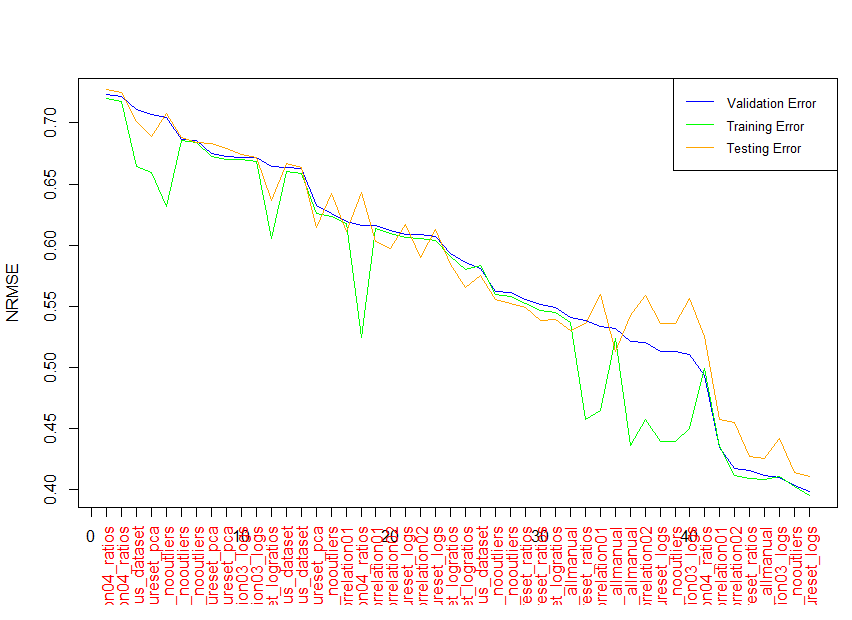
\includegraphics[width=0.95\linewidth]{img/exp01.png}
    \caption{Evolution of the NRMSE for the validation, training and testing set}\label{fig:Evol}
\end{figure}

% Summarized table
% latex table generated in R 3.4.3 by xtable 1.8-2 package
% 
\begin{table}[H]
\begin{tabular}{cllcc}
  \hline
 & subset[, 2] & Comment & Validation.NRMSE & Testing.NRMSE \\ 
  \hline
51 & regression\_randomforest & featureset\_logs & 0.40 & 0.41 \\ 
  56 & regression\_randomforest & featureset\_original\_nooutliers & 0.40 & 0.41 \\ 
  54 & regression\_randomforest & featureset\_nocorrelation03\_logs & 0.41 & 0.44 \\ 
  49 & regression\_randomforest & featureset\_allmanual & 0.41 & 0.43 \\ 
  59 & regression\_randomforest & featureset\_ratios & 0.42 & 0.43 \\ 
  53 & regression\_randomforest & featureset\_nocorrelation02 & 0.42 & 0.45 \\ 
  52 & regression\_randomforest & featureset\_nocorrelation01 & 0.43 & 0.46 \\ 
  55 & regression\_randomforest & featureset\_nocorrelation04\_ratios & 0.49 & 0.53 \\ 
  42 & regression\_tree\_rpartlib & featureset\_nocorrelation03\_logs & 0.51 & 0.56 \\ 
  39 & regression\_tree\_rpartlib & featureset\_logs & 0.51 & 0.54 \\ 
  44 & regression\_tree\_rpartlib & featureset\_original\_nooutliers & 0.51 & 0.54 \\ 
  41 & regression\_tree\_rpartlib & featureset\_nocorrelation02 & 0.52 & 0.56 \\ 
  37 & regression\_tree\_rpartlib & featureset\_allmanual & 0.52 & 0.54 \\ 
  25 & lasso regression GLMNET & featureset\_allmanual & 0.53 & 0.51 \\ 
  40 & regression\_tree\_rpartlib & featureset\_nocorrelation01 & 0.53 & 0.56 \\ 
  47 & regression\_tree\_rpartlib & featureset\_ratios & 0.54 & 0.54 \\ 
  13 & ridge regression GLMNET & featureset\_allmanual & 0.54 & 0.53 \\ 
  50 & regression\_randomforest & featureset\_logratios & 0.55 & 0.54 \\ 
  35 & lasso regression GLMNET & featureset\_ratios & 0.55 & 0.54 \\ 
  23 & ridge regression GLMNET & featureset\_ratios & 0.56 & 0.55 \\ 
  32 & lasso regression GLMNET & featureset\_original\_nooutliers & 0.56 & 0.55 \\ 
  20 & ridge regression GLMNET & featureset\_original\_nooutliers & 0.56 & 0.56 \\ 
  60 & regression\_randomforest & raw\_continuous\_dataset & 0.58 & 0.58 \\ 
  26 & lasso regression GLMNET & featureset\_logratios & 0.59 & 0.57 \\ 
  14 & ridge regression GLMNET & featureset\_logratios & 0.59 & 0.58 \\ 
  27 & lasso regression GLMNET & featureset\_logs & 0.61 & 0.61 \\ 
  29 & lasso regression GLMNET & featureset\_nocorrelation02 & 0.61 & 0.59 \\ 
  15 & ridge regression GLMNET & featureset\_logs & 0.61 & 0.62 \\ 
  17 & ridge regression GLMNET & featureset\_nocorrelation02 & 0.61 & 0.60 \\ 
  28 & lasso regression GLMNET & featureset\_nocorrelation01 & 0.62 & 0.60 \\ 
  43 & regression\_tree\_rpartlib & featureset\_nocorrelation04\_ratios & 0.62 & 0.64 \\ 
  16 & ridge regression GLMNET & featureset\_nocorrelation01 & 0.62 & 0.61 \\ 
  57 & regression\_randomforest & featureset\_pca\_nooutliers & 0.63 & 0.64 \\ 
  58 & regression\_randomforest & featureset\_pca & 0.63 & 0.61 \\ 
  36 & lasso regression GLMNET & raw\_continuous\_dataset & 0.66 & 0.66 \\ 
  24 & ridge regression GLMNET & raw\_continuous\_dataset & 0.66 & 0.67 \\ 
  38 & regression\_tree\_rpartlib & featureset\_logratios & 0.66 & 0.64 \\ 
  30 & lasso regression GLMNET & featureset\_nocorrelation03\_logs & 0.67 & 0.67 \\ 
  18 & ridge regression GLMNET & featureset\_nocorrelation03\_logs & 0.67 & 0.67 \\ 
  34 & lasso regression GLMNET & featureset\_pca & 0.67 & 0.68 \\ 
  22 & ridge regression GLMNET & featureset\_pca & 0.68 & 0.68 \\ 
  33 & lasso regression GLMNET & featureset\_pca\_nooutliers & 0.69 & 0.68 \\ 
  21 & ridge regression GLMNET & featureset\_pca\_nooutliers & 0.69 & 0.69 \\ 
  45 & regression\_tree\_rpartlib & featureset\_pca\_nooutliers & 0.70 & 0.71 \\ 
  46 & regression\_tree\_rpartlib & featureset\_pca & 0.71 & 0.69 \\ 
  48 & regression\_tree\_rpartlib & raw\_continuous\_dataset & 0.71 & 0.70 \\ 
  31 & lasso regression GLMNET & featureset\_nocorrelation04\_ratios & 0.72 & 0.72 \\ 
  19 & ridge regression GLMNET & featureset\_nocorrelation04\_ratios & 0.72 & 0.73 \\ 

   \hline
\end{tabular}
\label{experiments}\caption{Experiments performed and their NRMSE for validation and testing }

\end{table}

We also show in the fig.\ref{fig:Evol} how the mean of the normalized root mean squared error (NRMSE) when performing cross validation evolves in the different datasets, and compare it to how the training and test NRMSE performs.






% top 3 table
Our top 3 best performers consists of Random forest, Decision tree and Lasso regression models trained over feature datasets that contains logarithms of continuous variables, manually selected continuous vars that are not correlated between them or all the original dataset.
% latex table generated in R 3.4.3 by xtable 1.8-2 package
% 
\begin{table}[H]
\begin{tabular}{cllcc}
  \hline
 & Model & Dataset & Validation NRMSE & Testing NRMSE \\ 
  \hline
  51 & regression\_randomforest & featureset\_logs & 0.40 & 0.41 \\ 
  42 & regression\_tree\_rpartlib & featureset\_nocorrelation03\_logs & 0.51 & 0.56 \\ 
  25 & lasso regression GLMNET & featureset\_allmanual & 0.53 & 0.51 \\ 
  
   \hline
\end{tabular}
\label{experiments}\caption{Experiments performed and their NRMSE for validation and testing }
\end{table}


% forward selection explanation
Once we have found our best performing model and datasets, we run a forward selection algorithm to perform feature selection over each dataset with its corresponding model.\\

% forward selection table

%\scalebox{0.8}{

\begin{table}[H]
\centering
\resizebox{0.75\textwidth}{!}{
\begin{tabular}{cllcc}
  \hline
 & Model & Feature set & Validation.NRMSE & Testing.NRMSE \\ 
  \hline
1 & regression\_randomforest & featureset\_logs & 1.00 & 1.00 \\ 
  2 & regression\_randomforest & featureset\_logs 1\_7\_8\_13 & 0.98 & 0.98 \\ 
  3 & regression\_randomforest & featureset\_logs 1\_7\_8\_14 & 0.96 & 0.96 \\ 
  4 & regression\_randomforest & featureset\_logs 1\_7\_8\_15 & 0.99 & 1.00 \\ 
  5 & regression\_randomforest & featureset\_logs 1\_7\_8\_16 & 0.74 & 0.75 \\ 
  6 & regression\_randomforest & featureset\_logs 1\_7\_8\_17 & 0.83 & 0.81 \\ 
  7 & regression\_randomforest & featureset\_logs 1\_7\_8\_18 & 0.95 & 0.94 \\ 
  8 & regression\_randomforest & featureset\_logs 1\_7\_8\_19 & 0.82 & 0.83 \\ 
  9 & regression\_randomforest & featureset\_logs 1\_7\_8\_20 & 0.97 & 0.97 \\ 
  10 & regression\_randomforest & featureset\_logs 1\_7\_8\_16\_13 & 0.73 & 0.76 \\ 
  11 & regression\_randomforest & featureset\_logs 1\_7\_8\_16\_14 & 0.74 & 0.76 \\ 
  12 & regression\_randomforest & featureset\_logs 1\_7\_8\_16\_15 & 0.73 & 0.74 \\ 
  13 & regression\_randomforest & featureset\_logs 1\_7\_8\_16\_17 & 0.72 & 0.71 \\ 
  14 & regression\_randomforest & featureset\_logs 1\_7\_8\_16\_18 & 0.70 & 0.71 \\ 
  15 & regression\_randomforest & featureset\_logs 1\_7\_8\_16\_19 & 0.71 & 0.72 \\ 
  16 & regression\_randomforest & featureset\_logs 1\_7\_8\_16\_20 & 0.72 & 0.75 \\ 
  17 & regression\_randomforest & featureset\_logs 1\_7\_8\_16\_18\_13 & 0.70 & 0.71 \\ 
  18 & regression\_randomforest & featureset\_logs 1\_7\_8\_16\_18\_14 & 0.71 & 0.71 \\ 
  19 & regression\_randomforest & featureset\_logs 1\_7\_8\_16\_18\_15 & 0.71 & 0.73 \\ 
  20 & regression\_randomforest & featureset\_logs 1\_7\_8\_16\_18\_17 & 0.67 & 0.67 \\ 
  21 & regression\_randomforest & featureset\_logs 1\_7\_8\_16\_18\_19 & 0.69 & 0.69 \\ 
  22 & regression\_randomforest & featureset\_logs 1\_7\_8\_16\_18\_20 & 0.69 & 0.71 \\ 
  23 & regression\_randomforest & featureset\_logs 1\_7\_8\_16\_18\_17\_13 & 0.64 & 0.64 \\ 
  24 & regression\_randomforest & featureset\_logs 1\_7\_8\_16\_18\_17\_14 & 0.66 & 0.65 \\ 
  25 & regression\_randomforest & featureset\_logs 1\_7\_8\_16\_18\_17\_15 & 0.65 & 0.64 \\ 
  26 & regression\_randomforest & featureset\_logs 1\_7\_8\_16\_18\_17\_19 & 0.66 & 0.65 \\ 
  27 & regression\_randomforest & featureset\_logs 1\_7\_8\_16\_18\_17\_20 & 0.64 & 0.63 \\ 
  28 & regression\_randomforest & featureset\_logs 1\_7\_8\_16\_18\_17\_13\_14 & 0.63 & 0.63 \\ 
  29 & regression\_randomforest & featureset\_logs 1\_7\_8\_16\_18\_17\_13\_15 & 0.63 & 0.62 \\ 
  30 & regression\_randomforest & featureset\_logs 1\_7\_8\_16\_18\_17\_13\_19 & 0.63 & 0.62 \\ 
  31 & regression\_randomforest & featureset\_logs 1\_7\_8\_16\_18\_17\_13\_20 & 0.63 & 0.63 \\ 
  32 & regression\_randomforest & featureset\_logs 1\_7\_8\_16\_18\_17\_13\_15\_14 & 0.62 & 0.62 \\ 
  33 & regression\_randomforest & featureset\_logs 1\_7\_8\_16\_18\_17\_13\_15\_19 & 0.61 & 0.61 \\ 
  34 & regression\_randomforest & featureset\_logs 1\_7\_8\_16\_18\_17\_13\_15\_20 & 0.62 & 0.62 \\ 
  35 & regression\_randomforest & featureset\_logs 1\_7\_8\_16\_18\_17\_13\_15\_19\_14 & 0.60 & 0.60 \\ 
  36 & regression\_randomforest & featureset\_logs 1\_7\_8\_16\_18\_17\_13\_15\_19\_20 & 0.60 & 0.60 \\ 
  37 & regression\_randomforest & featureset\_logs 1\_7\_8\_16\_18\_17\_13\_15\_19\_20\_14 & 0.59 & 0.59 \\ 
   \hline

\end{tabular}

}
\caption{Execution of the forward selection algorithm }
\label{table:sfsranfomforest}
\end{table}
%}

In this table we can observe how we add features to the dataset until the validation error stops decreasing. At that point the best feature set is found. We can plot the evolution of the error measure (NRMSE of the cross validation) during the execution of the forward selection algorithm. In Figure.\ref{fig:rf_sfs} We can see the error in each iteration space (between the dashed-orange-lines), in every iteration we choose the feature that decrease the error the most.


\begin{figure}[H]
    \centering
        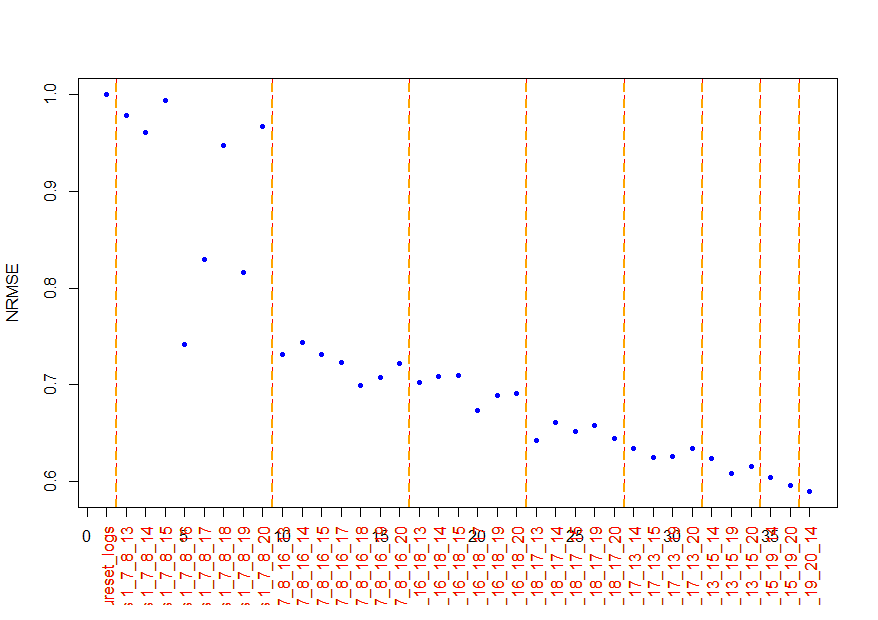
\includegraphics[width=0.8\textwidth]{img/randomForest.png}
    \caption{Evolution of the NRMSE for the Sequential forward selection}\label{fig:rf_sfs}
\end{figure}

We used SFS on the two best models, decision tree and lasso.
\textbf{Decision tree} - Using feature-set without correlated features gives us good results, knowing how decision tree this can be explained by the fact that every split will try to maximize the differences between it's nodes. When we are using features that are not correlate with each other it should help the model do better in it's splitting decision. We start the SFS with 8 features and add features iteratively. Eventually, the validation error dropped from 0.66 to 0.51.
\textbf{Lasso} - We used dataset with large range of features we extract. Start with the small number of features having validation error of 0.68, after 351 iteration of SFS algorithm, the final number of feature grow significantly and so the validation error dropped to 0.54.


%\scalebox{0.8}{
%% latex table generated in R 3.4.3 by xtable 1.8-2 package
% 
\begin{tabular}{cllcc}
  \hline
 & Model & Feature set & Validation.NRMSE & Testing.NRMSE \\ 
  \hline
1 & regression\_tree\_rpartlib & featureset\_nocorrelation03\_logs & 0.66 & 0.69 \\ 
  & ... & & ...& ... \\ 
  16 & regression\_tree\_rpartlib & featureset\_nocorrelation03\_logs 1\_2\_3\_4\_5\_6\_7\_8 & 0.51 & 0.56 \\ 
  & & \_10\_13\_9\_12\_11 & & \\
   \hline
\end{tabular}



%}\\
%\textbf{Forward selection of the decision tree model over the "featureset\_nocorrelation03\_logs" dataset:}\\


%\scalebox{0.8}{
%% latex table generated in R 3.4.3 by xtable 1.8-2 package
% 

\begin{tabular}{cllcc}
  \hline
 & Model & Feature set & Validation.NRMSE & Testing.NRMSE \\ 
  \hline
1 & lasso regression GLMNET & featureset\_allmanual & 0.68 & 0.66 \\ 
  2 & lasso regression GLMNET & featureset\_allmanual 1\_2\_3\_4\_5\_6\_7\_8\_9 & 0.68 & 0.65 \\ 
  & ... & & ... & ...\\
  351 & lasso regression GLMNET & featureset\_allmanual 1\_2\_3\_4\_5\_6 & 0.54 & 0.52 \\
   &  & \_7\_8\_16\_10\_13\_26\_28\_15\_30\_17\_18\_9 &  & \\ 
    &  & \_34\_20\_32\_35\_21\_14\_27\_19\_24\_33 &  & \\ 
   \hline
\end{tabular}


%}\\
%\textbf{Forward selection of the lasso model over the "featureset\_nocorrelation03\_logs" dataset:}\\


% forward selection plot




% explanation of the final fit
Once we have selected our best 3 models and performed feature selection over the dataset, we can fit the best model with the feature set and see what is its validation error and how it generalizes by the testing error.

% small resulting table of the final validatio errors


